%\chapter{\centerline{\Huge\textbf{ Synopsis}}}
\chapter{Synopsis}
\bigskip
\begin{quote}
\begin{tabular}[c]{ll}
Name: & {\textbf {Ravindra Kumar Verma}}\\
Roll No.: & {\textbf{ 13109883}}\\
Degree for which submitted: &  {\textbf{ Doctor of Philosophy}}\\
Department: & {\textbf{ Physics}}\\
Thesis Title: & {\textbf{ Search for a charged Higgs Boson at 13 TeV }}\\
 {}& {\textbf{ in the CMS experiment at the LHC, CERN}}\\
Thesis Supervisors: & {\textbf{ Prof. Pankaj Jain (IIT Kanpur),}}\\ 
{}&{\textbf{ Prof. Shashi R. Dugad (TIFR Mumbai)}}\\ 
Month and year of submission: & {\textbf{ August 2019}} 
\end{tabular}
\end{quote}
\hrulefill
\bigskip

The discovery of the Higgs boson in 2012 by the ATLAS and CMS experiments at 
the CERN LHC has ushered a new beginning in the field of particle physics. 
The Higgs boson could be the first of many elementary scalars present in 
nature to be observed in the laboratory. Various extensions to the standard 
model (SM), such as supersymmetry and the two Higgs doublet model (2HDM), 
predict multiple scalars as the remnants of an additional SU(2)$_L$ complex 
doublet introduced to address some known drawbacks of the SM. After spontaneous 
symmetry breaking, out of the eight degrees of freedom of the two Higgs doublets, 
three are used to make the \PW and \PZ bosons massive, leaving five physical scalar
particles. Of these, two (\Ph, \PH) are neutral Higgs bosons which are
CP-even (scalar), one (\PSA) is neutral and CP-odd (pseudoscalar), and the
remaining two are charged Higgs \PHpm bosons.

The 2HDM can be classified into different categories depending on the type of
interaction of the two doublets with quarks and charged leptons. For example,
in the type I 2HDM, fermions have Yukawa couplings only to the second doublet.
The nature of the Yukawa coupling determines the branching fraction of the charged
Higgs boson decays into different final states. In this thesis, a search for the
charged Higgs boson has been performed in the decay channel $\Hp \to \PQc\PAQs$ (and 
its charge conjugate), whose branching fraction 
can range anywhere up to 100\% depending on the type of Yukawa couplings. The 
latter is expressed in terms of the parameter $\tan\beta=v_2/v_1$ where $v_1$ 
and $v_2$ are the vacuum expectation values of the two Higgs doublets. In the 
minimal supersymmetric standard model (MSSM), this is the dominant decay channel 
for low values of $\tan\beta$. In this thesis, we perform a model-independent search for the charged Higgs boson assuming that $\mathcal{B}(\Hp \to \PQc\PAQs) = 100$\%. 

Limits on charged Higgs boson production at hadron colliders have been set by the 
Tevatron and LHC, assuming the production mode $\PQt \to \Hp\PQb$. The CDF 
collaboration set a 95\% \CL upper limit on the branching 
fraction $\mathcal{B}(\PQt \to \Hp\PQb) < 10$--30\% for a charged Higgs lying in 
the mass range 60--150\GeV, assuming that $\Hp$ decays dominantly to $\PQc\PAQs$. 
Similar limits have been obtained by the D0 experiment. 
Using the 7\TeV data, the ATLAS collaboration set an upper limit at 95\% \CL on 
the product $\mathcal{B}(\PQt \to \Hp\PQb) \mathcal{B}(\Hp \to \PGtp\PGn) < 
0.23$--1.3\% for a charged Higgs mass in the range 80--160\GeV. 
A search for a charged Higgs boson decaying into $\PQc\PAQs$ was performed at 
8\TeV by the CMS collaboration, which set an upper limit at 95\% \CL on 
$\mathcal{B}(\PQt \to \Hp\PQb)$ in the range 1.2--6.5\%. In this thesis, 
the analysis of collision data recorded in 2016 by the CMS experiment at 13\TeV
is presented.  

As illustrated in Figure~\ref{fig:feyn_diag_sig}, the principal SM background to 
this search consists of \ttbar pair production where one of the top quarks decays 
by $\PQt \to \PWp\PQb$ and the other top quark decays by $\PAQt \to \PWm\PAQb$; 
this is referred to as the \dq{semileptonic} decay channel. In contrast, in the signal
process, one of the top quarks decays to $\Hp\PQb$ and the other to $\PWm\PAQb$. 
The $\PWp/\Hp$ decays hadronically into \dq{light} jets (not from a \PQb quark), 
whereas the \PWm decays leptonically. We define two channels depending on whether 
the lepton produced in the \PWm decay is an electron or a muon (events with tau 
leptons are not considered).
\begin{figure}[htp]
\begin{center}
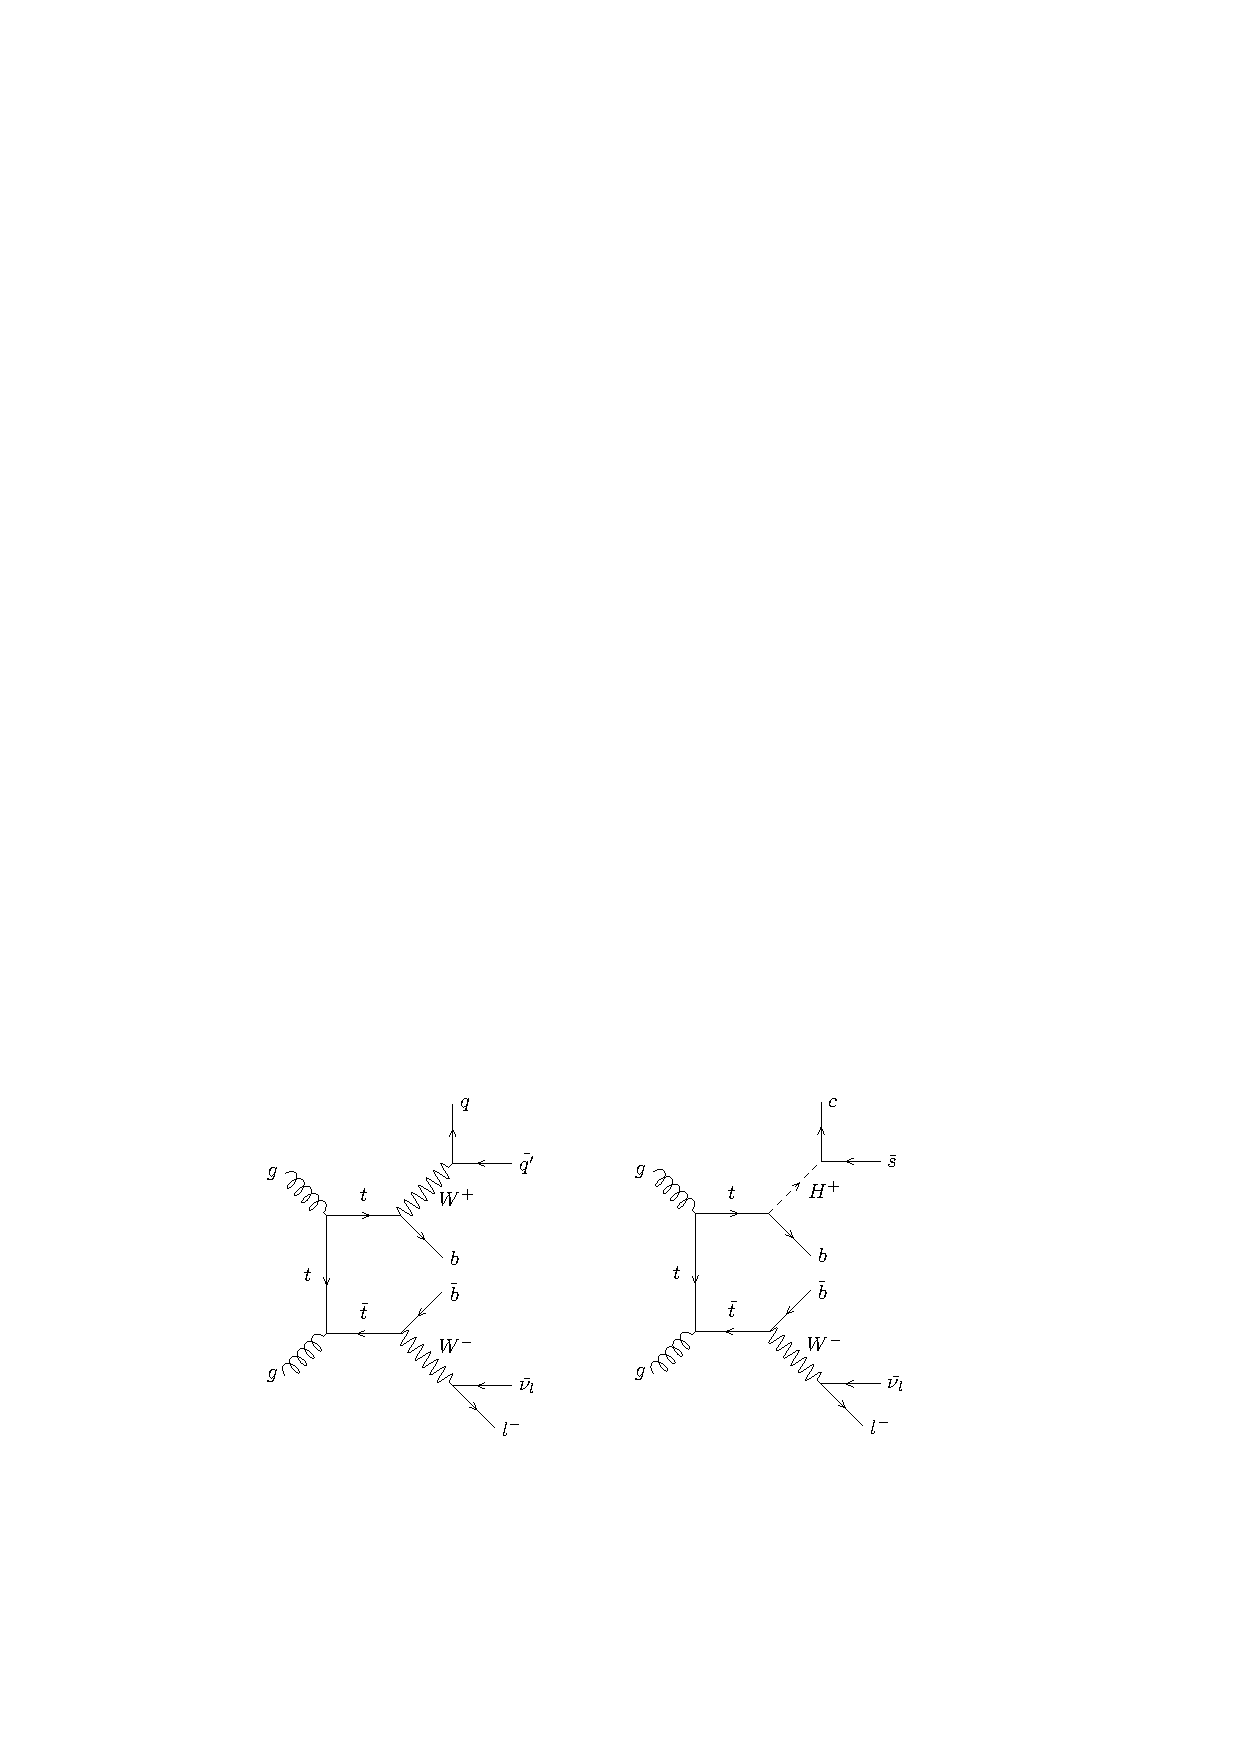
\includegraphics[width=0.75\textwidth]{University/Image/Synopsis/feyn_diag_sig.pdf}
\caption{Production of \ttbar from gluon-gluon scattering. The left plot shows
the SM decay of the \ttbar pair in the semileptonic decay channel. The right plot 
shows the signal process in which the \ttbar pair decay products include a charged Higgs boson.}
\label{fig:feyn_diag_sig}
\end{center}
\end{figure}

\section*{Summary of research work}
In \textbf{chapter 1}, we present a brief theoretical overview of the standard model of
particle physics where we discuss it's successes and failures. In \textbf{chapter 2}, the
two Higgs doublet model is described where various properties of the charged Higgs such
as it's interaction with the particles of SM are discussed. In the same chapter,
we present the current status of the charged Higgs searches and the search strategy followed
in this thesis.

In \textbf{chapter 3}, we present a brief description of the LHC and the detectors
installed there. A few important parameters of the LHC have also been described along
with a few physics parameters. In \textbf{chapter 4}, a brief overview of the CMS
experiment is presented. \quotes{ The central feature of the CMS apparatus is a superconducting 
solenoid of 6\unit{m} internal diameter, providing a magnetic field of 3.8\unit{T}. 
Within the solenoid volume are a silicon pixel and strip tracker, a lead tungstate 
crystal electromagnetic calorimeter (ECAL), and a brass and scintillator hadron 
calorimeter (HCAL), each composed of a barrel and two endcap sections. Silicon pixel 
and tracker detector identifies the trajectory of charged particles and accurately 
measures their transverse momentum up to $|\eta| \leq 2.5$.  Forward calorimeters 
extend the pseudorapidity coverage provided by the barrel and endcap calorimeter. 
Segmented calorimeters provide sampling of electromagnetic and hadronic showers 
up to $|\eta| \leq 5$. Muons are detected in gas-ionization chambers embedded in 
the steel flux-return yoke outside the solenoid in the range of $|\eta| \leq 2.4$}. 

In \textbf{chapter 5}, we list the collision and simulated data samples. The data 
used for the analysis was collected by the CMS detector in 2016 in proton-proton 
($\Pp\Pp$) collisions at $\sqrt{s}$ = 13\TeV, with an integrated luminosity of 35.9\fbinv.  
The simulated signal and background samples are generated using the \MGvATNLO and \POWHEG v2 
generators at parton level. In all cases, these parton level events are hadronized 
using \PYTHIA 8 with the CUETP8M1 tune, and then passed to \GEANTfour for simulation of 
the CMS detector response. In the same chapter, we describe the reconstruction and
identification of various physics objects.  

In \textbf{chapter 6}, we describe various corrections applied on simulated samples.
In \textbf{chapter 7}, the event selection has been described. In the event 
topology of interest, there are four jets (two \PQb jets and two light jets), 
one charged lepton, and missing transverse energy. Various selection requirements are 
applied to ensure the resulting events have this topology. 

In \textbf{chapter 8}, we perform kinematic fitting to select events coming from
true \ttbar decay. In this analysis, the charged Higgs boson is assumed to decay 
to $\PQc\PAQs$. The invariant mass of the system of the two light jets (\mjj) is 
thus used as the final observable. If the two observed light jets come from a 
semileptonic \ttbar decay, then the \mjj distribution should have a peak at the 
\PW boson mass. However, the observed mean of the \mjj distribution is much higher 
(around 128 \GeV), reflecting the fact that the two light jets in each event may 
not necessarily come from the decay of a \PW boson. To select true semileptonic
\ttbar events, a kinematic fit is performed on the reconstructed objects using 
the top quark kinematic fitter package. In the output, the top quark  
kinematic fitter gives exactly four jets (two \PQb jets, one from each of the 
leptonic and hadronic \PQt decays, and two light jets from the hadronic \PQt 
decay), a lepton, and a neutrino. The two light jets coming from the hadronic 
\PQt decay are further used for charm tagging. 

In \textbf{chapter 9}, we describe the procedure to estimate QCD multijet background from data.
The simulation of QCD multijet events is computationally intensive, resulting in a 
limited number of such events being available. A data-driven approach is used 
to make a more precise estimation of the QCD multijet background.

In \textbf{chapter 10}, the \mjj distribution without and with charm quark tagging 
is presented. Further, events are divided exclusively into loose, medium, and tight 
categories, based on whether at least one of the light jets passes the loose 
but neither passes the medium, at least one passes the medium but neither passes 
the tight, or at least one passes the tight working points of the charm tagging 
selection requirements, respectively. The expected signal to background ratio 
is different in the various charm categories, so partitioning the events into 
categories results in an improvement in the expected upper limits on \brThb. 

In \textbf{chapter 11}, a detailed description of the statistical and systematic
uncertainties is given. There are various sources of systematic uncertainty which may 
arise due to detector calibration effects, uncertainty in the measured reconstructed 
efficiency, the theoretical modeling of signal events, and other effects. 

In \textbf{chapter 12}, the final results are presented. The total expected background number 
of events agrees with the data within uncertainties. The absence of a charged Higgs 
signal in the data is characterized by setting exclusion limits on the branching ratio 
\brThb, assuming that $\mathcal{B}(\Hp \to \PQc\PAQs)$ = 100\%. 
In the absence of any excess, an asymptotic 95\% confidence level (\CL) limit using 
the likelihood ratios on \brThb is calculated. 

In \textbf{chapter 13}, we conclude the analysis. We also discuss the future 
aspects of the analysis and how the current experimental results can be interpreted 
in different types of the two Higgs doublet model. 



